
Use case modeling, which is mostly used to model interactions between a system and external agents (human users or other systems).


\subsection{Use-case diagrams}

\begin{figure}[H]
\begin{center}

	\tcbox{\includegraphics[width=10cm]{{"Diagram/Manage Account"}.png}}
	\caption{Use-case diagram for Manage account}
	\label{dia_uscs_mng_acnt}

\end{center}
\end{figure}

\begin{figure}[H]
\begin{center}

	\tcbox{\includegraphics[width=10cm]{{"Diagram/Manage Content"}.png}}
	\caption{Use-case diagram for Manage content}
	\label{dia_uscs_mng_cntnt}

\end{center}
\end{figure}

\begin{figure}[H]
\begin{center}	

	\tcbox{\includegraphics[width=15cm]{{"Diagram/Manage User"}.png}}
	\caption{Use-case diagram for Manage User}
	\label{dia_uscs_mng_usr}

\end{center}
\end{figure}

\begin{figure}[H]
\begin{center}	

	\tcbox{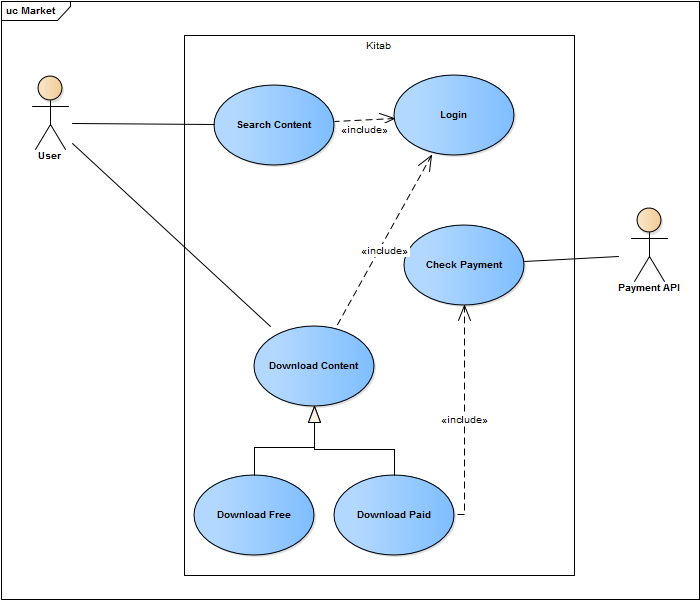
\includegraphics[width=15cm]{Diagram/Market.png}}
	\caption{Use-case diagram for Market}
	\label{dia_uscs_mrkt}

\end{center}
\end{figure}

\begin{figure}[H]
\begin{center}	

	\tcbox{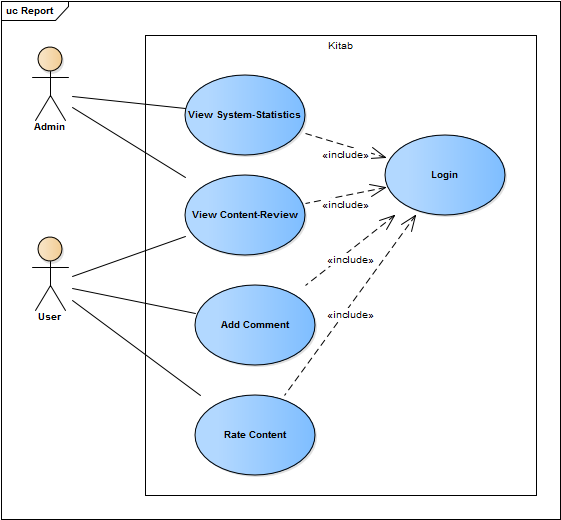
\includegraphics[width=15cm]{Diagram/Report.png}}
	\caption{Use-case for Report}
	\label{dia_uscs_rprt}

\end{center}
\end{figure}
